\begin{figure}[!htb]
\begin{center}
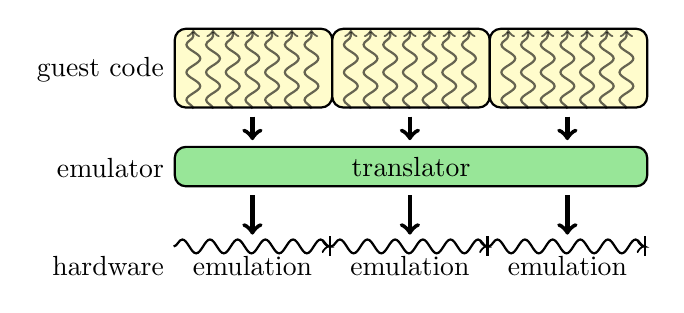
\begin{tikzpicture}

\node at (0,2.5) [left] {guest code};
\node at (0,2) [rectangle, draw=black, thick, rounded corners, fill=yellow!20,  minimum height = 1cm, minimum width = 2cm, anchor=south west] (b1) {};
\begin {scope} [opacity=0.6]
\draw[thick, decorate, decoration=snake, ->] (0.25, 2) -- (0.25, 3);
\draw[thick, decorate, decoration=snake, ->] (0.5, 2) -- (0.5, 3);
\draw[thick, decorate, decoration=snake, ->] (0.75, 2) -- (0.75, 3);
\draw[thick, decorate, decoration=snake, ->] (1, 2) -- (1, 3);
\draw[thick, decorate, decoration=snake, ->] (1.25, 2) -- (1.25, 3);
\draw[thick, decorate, decoration=snake, ->] (1.5, 2) -- (1.5, 3);
\draw[thick, decorate, decoration=snake, ->] (1.75, 2) -- (1.75, 3);
\end {scope}

\node at (2,2) [rectangle, draw=black, thick, rounded corners, fill=yellow!20, minimum height = 1cm, minimum width = 2cm, anchor=south west] (b2) {};
\begin {scope} [opacity=0.6]
\draw[thick, decorate, decoration=snake, ->] (2.25, 2) -- (2.25, 3);
\draw[thick, decorate, decoration=snake, ->] (2.5, 2) -- (2.5, 3);
\draw[thick, decorate, decoration=snake, ->] (2.75, 2) -- (2.75, 3);
\draw[thick, decorate, decoration=snake, ->] (3, 2) -- (3, 3);
\draw[thick, decorate, decoration=snake, ->] (3.25, 2) -- (3.25, 3);
\draw[thick, decorate, decoration=snake, ->] (3.5, 2) -- (3.5, 3);
\draw[thick, decorate, decoration=snake, ->] (3.75, 2) -- (3.75, 3);
\end {scope}

\node at (4,2) [rectangle, draw=black, thick, rounded corners, fill=yellow!20, minimum height = 1cm, minimum width = 2cm, anchor=south west] (b2) {};
\begin {scope} [opacity=0.6]
\draw[thick, decorate, decoration=snake, ->] (4.25, 2) -- (4.25, 3);
\draw[thick, decorate, decoration=snake, ->] (4.5, 2) -- (4.5, 3);
\draw[thick, decorate, decoration=snake, ->] (4.75, 2) -- (4.75, 3);
\draw[thick, decorate, decoration=snake, ->] (5, 2) -- (5, 3);
\draw[thick, decorate, decoration=snake, ->] (5.25, 2) -- (5.25, 3);
\draw[thick, decorate, decoration=snake, ->] (5.5, 2) -- (5.5, 3);
\draw[thick, decorate, decoration=snake, ->] (5.75, 2) -- (5.75, 3);
\end {scope}

\draw[ultra thick, ->] (1, 1.9) -- (1, 1.6);
\draw[ultra thick, ->] (3, 1.9) -- (3, 1.6);
\draw[ultra thick, ->] (5, 1.9) -- (5, 1.6);
\draw[ultra thick, ->] (1, 0.9) -- (1, 0.4);
\draw[ultra thick, ->] (3, 0.9) -- (3, 0.4);
\draw[ultra thick, ->] (5, 0.9) -- (5, 0.4);

\node at (0,1) [rectangle, draw=black, thick, rounded corners,  fill=LimeGreen!50, minimum height = 0.5cm, minimum width = 6cm, anchor=south west] (tr) {translator};
\node at (0,1.25) [left] {emulator};

\node at (0,0) [left] {hardware};
\draw[thick, decorate, decoration=snake, ->|] (0, 0.25) -- (2, 0.25)  node [below, align=center, midway, text width=2cm] {emulation};
\draw[thick, decorate, decoration=snake, ->|] (2, 0.25) -- (4, 0.25)  node [below, align=center, midway, text width=2cm] {emulation};
\draw[thick, decorate, decoration=snake, ->|] (4, 0.25) -- (6, 0.25)  node [below, align=center, midway, text width=2cm] {emulation};

\end{tikzpicture}
\end{center}
\ifreport
\caption{Software-based Virtualization}
\fi
\label{fig-virt-software}
\end{figure}
